\documentclass[12,french]{report}
\usepackage{geometry}
\geometry{vmargin=3cm, hmargin=3cm}
\usepackage[T1]{fontenc}
\usepackage[utf8]{inputenc}
\usepackage[french]{babel}
\usepackage{graphicx}
\usepackage{amsmath}
\usepackage{amssymb}
\usepackage{sectsty}
\usepackage{authblk}
\usepackage{algpseudocode}
\usepackage{algorithm}
\usepackage{xspace}
\usepackage{mathtools}
\usepackage{mathrsfs}
\usepackage{enumitem}
\usepackage{titlesec}
\usepackage{hyperref}
\usepackage{xcolor}
\usepackage{caption}
\usepackage{float}
\usepackage{tabto}

\usepackage{listings}
\usepackage{cleveref}

\renewcommand{\lstlistingname}{Code}
%\renewcommand{\figurename}{Fig.}

\lstdefinestyle{chstyle}{%
backgroundcolor=\color{gray!12},
basicstyle=\ttfamily\small,
showstringspaces=false,
numbers=left}

%\AddThinSpaceBeforeFootnotes
%\FrenchFootnotes

\titleformat{\chapter}[hang]{\bf\Huge}{\thechapter.}{2pc}{}
\titlespacing*{\chapter}{10pt}{0pt}{40pt}[0pt]
\newcommand{\HRule}{\rule{\linewidth}{0.5mm}}

\providecommand{\keywords}[1]{\textbf{\textit{Keywords:}} #1}
\bibliographystyle{apalike}

\usepackage{hyperref}

\begin{document}
\hypersetup{pdfborder=0 0 0}

\begin{titlepage}

\begin{center}
	\vspace*{\stretch{1}}
	\textsc{{\LARGE Institut national des sciences appliquées de Rouen} \\ 			\vspace{6mm} {\Large INSA de Rouen}} \\
	\vspace{5mm}
	
\includegraphics[width=0.4\textwidth]{./Images/insa}\\[1.0 cm]

	\textsc{\Large Projet Info GM3 - Vague 1 - Sujet 2}\\[0.6cm]

	% Title
	\HRule \\[0.5cm]
	{ \Huge \bfseries Simulation d'une loi exponentielle de paramètre $\lambda$}\\[0.2cm]
	\HRule \\[0.95cm]

	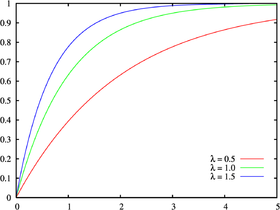
\includegraphics[width=0.6\textwidth]{./Images/Courbes_loi_exp}\\[0.9 cm]

	% Author and supervisor
	\begin{minipage}{0.4\textwidth}
		\begin{flushleft} \large
			\emph{Auteurs:}\\
			Thibaut \textsc{André-Gallis} \\
			{\small\href{mailto:thibaut.andregallis@insa-rouen.fr}{thibaut.andregallis@insa-rouen.fr}} \\
			Kévin \textsc{Gatel} \\
			{\small\href{mailto:kevin.gatel@insa-rouen.fr}{kevin.gatel@insa-				rouen.fr}}
		\end{flushleft}
	\end{minipage}
	\begin{minipage}{0.4\textwidth}
		\begin{flushright} \large
			\emph{Enseignant:} \\
			Ioana \textsc{Ciotir} \\
			{\small\href{mailto:ioana.ciotir@insa-rouen.fr}								{ioana.ciotir@insa-rouen.fr}}
		\end{flushright}
	\end{minipage}
	\vspace*{\stretch{1}}

	\vfill
	{\large 27 Novembre 2020}
\end{center}
\end{titlepage}

\tableofcontents

%\listoffigures

\renewcommand{\chaptername}{}
\chapter*{Introduction}
%\label{chapter:Introduction}
\addcontentsline{toc}{chapter}{Introduction}

La loi exponentielle modélise la durée de vie d'un phénomène sans mémoire ou sans vieillissement. En d'autres termes la probabilité que le phénomène dure au moins $h+t$ heures sachant qu'il a déjà duré $t$ heures sera la même que la probabilité de durer $h$ heures à partir de sa mise en fonction initiale. Elle peut notamment modéliser la vie des circuits électriques, résoudre des problématiques de durée de vie en général.\\

Dans ce projet nous allons nous intéresser à comment simuler et modéliser une loi exponentielle de paramètre $\lambda$. Dans un premier temps nous allons démontrer qu'il est possible d'obtenir une loi exponentielle $G(U)$ en partant d'une loi uniforme $U$, ensuite nous allons démontrer que prendre une loi uniforme $U$ ou bien $1-U$ ne change rien pour en obtenir une. Dans un deuxième nous allons vérifier expérimentalement qu'il est possible de générer une loi exponentielle à partir d'une loi uniforme et vérifier que $G(U) \sim G(1-U)$.

\chapter{Partie théorique}

Dans cette partie, nous allons démontrer les deux premières questions posées.

\section{G(U) $\sim$ $\varepsilon(\lambda)$}

Soit $U$ une loi uniforme sur [0,1].

On a :

$$\mathbb{P}(U\leq t)=F_{U}(t)=\begin{cases}
0 & \text{si \ensuremath{t<0} }\\
\frac{t-0}{1-0}=t & \text{si \ensuremath{t}}\in[0,1]\\
1 & \text{si \ensuremath{t>1}}
\end{cases}$$

Soit $\lambda>0$ et $G$ une fonction telle que : \\

$$\begin{array}{ccccc}
	G & : & [0,1] & \longrightarrow & \mathbb{R}^{+} \\
	& & u & \longmapsto & \frac{-1}{\lambda}\ln(1-u) \\
\end{array}$$

Alors : \\
$$\mathbb{P}(G(U)<t)=\mathbb{P}(\frac{-1}{\lambda}\ln(1-U)<t)=\mathbb{P}(\ln(1-U)>-\lambda t)=\mathbb{P}(1-U>e^{-\lambda t})$$
Or :
$$\mathbb{P}(1-U>e^{-\lambda t})=\mathbb{P}(U<1-e^{-\lambda t})=F_{U}(1-e^{-\lambda t})=\begin{cases}
0 & \text{si \ensuremath{1-e^{-\lambda t}<0}}\\
1-e^{-\lambda t} & \text{si \ensuremath{\ensuremath{1}-}\ensuremath{e^{-\lambda t}}}\in[0,1]\\
1 & \text{si \ensuremath{1-e^{-\lambda t}>1}}
\end{cases}$$

On a :
$$\begin{array}{ccl}
	1-e^{-\lambda t}<0 & \iff & e^{-\lambda t}>1 \\
					   & \iff & \underbrace{-\lambda}_{<0}t>0 \\
					   & \iff & t<0 \\
\end{array}$$\\

Ensuite :
$$\begin{array}{ccl}
	1-e^{-\lambda t}\in[0,1] & \iff & 0\leq1-e^{-\lambda t}\leq1 \\
					   & \iff & e^{-\lambda t}\leq1 \\
					   & \iff & \underbrace{-\lambda}_{<0}t\leq0 \\
					   & \iff & t\geq0 \\
\end{array}$$\\

Enfin :
$$\begin{array}{ccl}
	1-e^{-\lambda t}>1 & \iff & e^{-\lambda t}<0 \\
	& \iff & t\in\emptyset \\
  \end{array}$$\\
  
Ainsi :
$$\mathbb{P}(G(U)<t)=\begin{cases}
0 & \text{si \ensuremath{t<0}}\\
1-e^{-\lambda t} & \text{si }t\geq0
\end{cases}$$\\

D'où $G(U) \sim \varepsilon(\lambda)$.\vspace{0.4cm}
 
\section{G(U) $\sim$ G(1-U) $\sim$ $\varepsilon(\lambda)$}

On a :
$$\mathbb{P}(G(1-U)<t)=\mathbb{P}(\frac{-1}{\lambda}\ln(U)<t)=\mathbb{P}(\ln(U)>-\lambda t)$$\\
D'où : $$\mathbb{P}(\ln(U)>-\lambda t)=\mathbb{P}(U>e^{-\lambda t})=1-\mathbb{P}(U<e^{-\lambda t})=1-F_{U}(e^{-\lambda t})$$\\

Or : $$F_{U}(e^{-\lambda t})=\begin{cases}
0 & \text{si \ensuremath{e^{-\lambda t}<0}}\text{ Aucun t ne satisfait l'inéquation }\\
e^{-\lambda t} & \text{si \ensuremath{e^{-\lambda t}}}\in[0,1]\\
1 & \text{si \ensuremath{e^{-\lambda t}>1}}
\end{cases}$$\\
Donc :
$$-F_{U}(e^{-\lambda t})=\begin{cases}
-e^{-\lambda t} & \text{si \ensuremath{-}\ensuremath{e^{-\lambda t}}}\in[-1,0]\\
-1 & \text{si \ensuremath{-e^{-\lambda t}<-1}}
\end{cases}$$\\
Enfin :
$$1-F_{U}(e^{-\lambda t})=\mathbb{P}(G(1-U)<t)=\begin{cases}
1-e^{-\lambda t} & \text{si \ensuremath{1-}\ensuremath{e^{-\lambda t}}}\in[0,1]\iff t\geq0\\
0 & \text{si \ensuremath{1-e^{-\lambda t}<0}\ensuremath{\iff t<0}}
\end{cases}=F_{U}(1-e^{-\lambda t})$$\\

On retombe bien sur la même loi exponentielle que $G(U)$. \\

Pour conclure si $U\sim\mathbb{U}([0,1])$ on aura $G(1-U) \sim G(U)\sim \varepsilon(\lambda)$.

\chapter{Partie appliquée}

Dans cette partie nous allons illustrer ce que nous venons de démontrer en construisant un exemple. Nous avons ainsi fait un programme qui, en partant d'une simple loi uniforme que possèdent les langages traditionnels, génère une loi exponentielle\footnote{Le code est disponible en annexe}. Nous allons ensuites analyser ces résultats afin de discuter de la méthode et de la conformité.\\

\section{Construction et analyse de l'exemple}

Dans un premier temps nous avons tiré puis stocké un grand nombre de valeurs (ici $N$=2000) tirées aléatoirement de manière uniforme entre [0,1]. La fonction $G$ est appliquée au tableau puis ce dernier est trié de manière à classer par ordre croissant les valeurs. Nous avons ensuite utilisé un second tableau compteur permettant de comptabiliser  le nombre de valeur inférieur à seconde valeur constante appartenant au tableau créé précédemment. Enfin, en incrémentant cette constante on peut ainsi construire une fonction de répartition de nos valeurs tirées initialement de manière aléatoire. On trace ensuite les deux courbes pour pouvoir les comparer. Pour pouvoir comparer notre résultat obtenu à la courbe théorique afin de valider notre simulation, nous avons tracé la fonction de répartition d'une loi exponentielle de paramètre $\lambda$ nous servant ainsi de modèle.\\

On obtient ce résultat :

\begin{figure}[H]
    \begin{minipage}[c]{.50\linewidth}
        \centering
        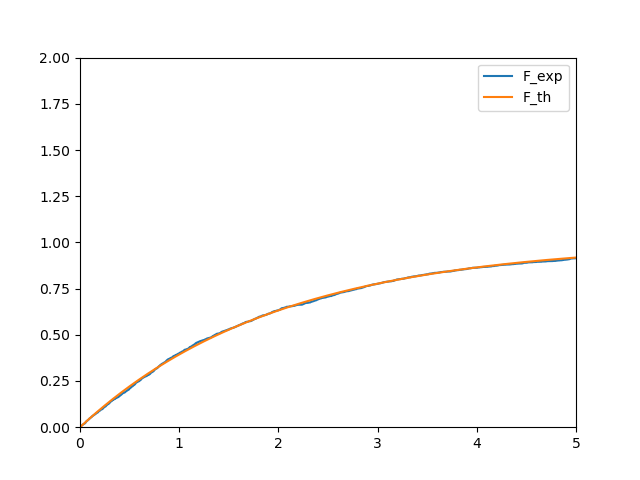
\includegraphics[width=0.9\textwidth]{./Images/Lambda_0.5}\\
        \caption*{Fonction de répartition avec $\lambda=0.5$}
    \end{minipage}
    \hfill%
    \begin{minipage}[c]{.50\linewidth}
        \centering
        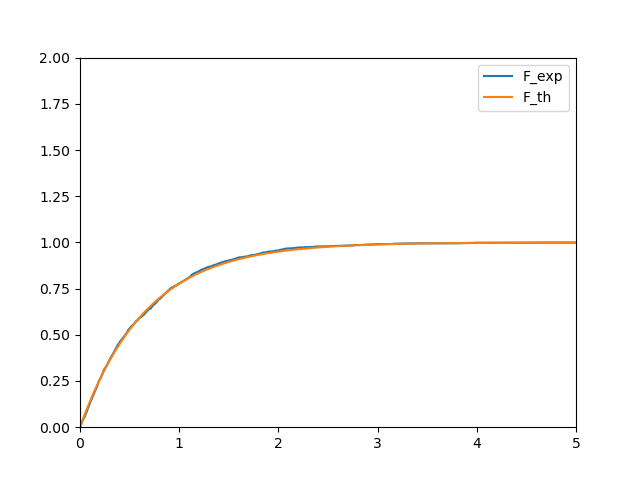
\includegraphics[width=0.9\textwidth]{./Images/Lambda_1.5}\\
        \caption*{Fonction de répartition avec $\lambda=1.5$}
    \end{minipage}
\end{figure}\vspace{0.3cm}

On obtient des courbes très proches voire superposées ce qui est bon signe.\\

Pour avoir d'autres éléments à étudier, nous avons comparé l'espérance obtenue avec celle théorique. \\

\begin{minipage}{0.5\textwidth}
		\begin{flushleft} \large\center
			Pour $\lambda$=0.5 \vspace{0.4cm}
			
				\begin{tabular}{|l|c|}
 				\hline
			    $\mathbb{E}_{th}$ & $\mathbb{E}_{exp}$ \\
    			\hline
   				$2$ & $2.01158$ \\
   				\hline
   				\end{tabular}
		\end{flushleft}
	\end{minipage}
	\begin{minipage}{0.4\textwidth}
		\begin{flushright} \large\center
			Pour $\lambda$=1.5 \vspace{0.4cm}
			
				\begin{tabular}{|l|c|r|}
				\hline
			    $\mathbb{E}_{th}$ & $\mathbb{E}_{exp}$ \\
    			\hline
   				$0.66667$ & $0.67476$ \\
   				\hline
   				\end{tabular}
		\end{flushright}
	\end{minipage}\vspace{0.5cm}

Les espérances sont également très proches.
On calcule aussi numériquement l'écart moyen entre les deux courbes en plus du tracé de la courbe. On obtient ainsi :\\

\begin{minipage}{0.5\textwidth}
		\begin{flushleft} \large\center
			Pour $\lambda$=0.5 \vspace{0.4cm}
			
				\begin{tabular}{|l|c|}
 				\hline
			    Ecart \\
    			\hline
   				0.00963\\
   				\hline
   				\end{tabular}
		\end{flushleft}
	\end{minipage}
	\begin{minipage}{0.4\textwidth}
		\begin{flushright} \large\center
			Pour $\lambda$=1.5 \vspace{0.4cm}
			
				\begin{tabular}{|l|c|r|}
				\hline
			    Ecart \\
    			\hline
   				0.00557\\
   				\hline
   				\end{tabular}
		\end{flushright}
	\end{minipage}\vspace{0.5cm}

Nous retrouvons bien toutes les propriétés d'une loi exponentielle. La loi exponentielle formée par $G(U)$ est donc bien vérifiée expérimentalement.\\

\section{Cohérence de $U$ et $1-U$ pour $G$}

Pour ce faire, nous avons fabriqué de la même manière la fonction de répartition en prenant $1-U$ au lieu de $U$.\\

Nous obtenons :

\begin{figure}[H]
	\center
	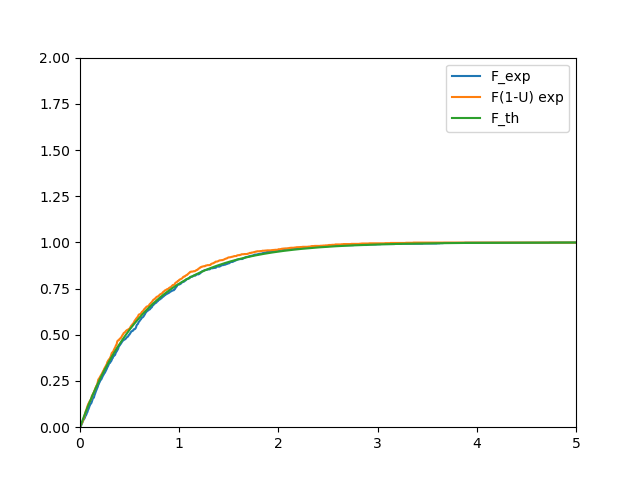
\includegraphics[width=0.92215\textwidth]{./Images/EcartU}
	\caption{Fonctions de répartition}
\end{figure}\vspace{0.2cm}

Nous observons que les deux courbes ont la même allure et sont très proches. De plus nous obtenons cette figure avec une moyenne des écarts entre les deux courbes expérimentales de l'ordre de 1\%

\begin{center}
\begin{tabular}{|l|c|r|}
				\hline
			    Ecart \\
    			\hline
   				$0.01038$\\
   				\hline
   				\end{tabular}
\end{center}

Ainsi, nous pouvons donc conclure sur la cohérence de $U$ et $1-U$ pour la fonction $G$.

\chapter*{Conclusion}
\addcontentsline{toc}{chapter}{Conclusion}

Pour conclure ce projet rappelons le problème initial. Nous avons donc étudié la loi exponentielle de paramètre lambda d'un point de vue mathématique et informatique. Pour ce faire nous avons simulé une loi exponentielle à partir d'une loi uniforme. Ce projet a donc été réalisé en deux partie : une mathématique et une plus informatique.\\

En première partie on s'est intéresse à l'aspect purement mathématique. Nous disposions d'une certaine fonction G tel que :
$$\begin{array}{ccccc}
	G & : & [0,1] & \longrightarrow & \mathbb{R}^{+} \\
	& & u & \longmapsto & \frac{-1}{\lambda}\ln(1-u) \\
\end{array}$$ 
Et d'une variable aléatoire U suivant une loi uniforme sur [0,1]. Nous avons donc démontré mathématiquement que la variable G(U) suivait une loi exponentielle de paramètre $\lambda$. Nous avons ensuite démontrer que si l'on remplaçait U par 1-U dans G on trouvait le même résultat.\\

Dans un second temps nous avons essayé d'implémenter un programme informatique permettant d'illustrer cette démonstration à travers un exemple. Nous savions que la plupart des langages possèdent une fonction aléatoire qui suit une loi uniforme sur [0,1]. Notre programme consiste à faire de  nombreux tirages aléatoires indépendant en nous servant de cette fonction et de la fonction G. Les valeurs tirées sont stockés dans un tableau. Pour ensuite vérifier que ces valeurs suivaient bien une loi exponentielle de paramètre $\lambda$, nous avons eu l'idée de tracer la fonction de répartition de ces valeurs et de la comparer avec la fonction de répartition théorique. Nous ne nous sommes pas contenté de ça et nous avons aussi comparé l'espérance de nos mesures et l'espérance théorique. Nous avons ensuite réitéré l'expérience avec la variable 1-U et constaté la même chose.\\

Nous avons eu des difficultés pour obtenir une courbe lisse avec un nombre fini de valeurs mais nous avons finalement trouvé un bon équilibre permettant d'obtenir une courbe de bonne qualité très proche de la courbe théorique sans surcharger l'utilisation de la mémoire et le nombre d'opérations qui rendait le programme très long à s'exécuter.\\

Pour finir ce projet nous aura permis de nous familiariser avec un langage supplémentaire qu'est le python, ainsi que des logiciels comme numpy très utile pour tracer des graphiques.\\

Nous avons trouvé très intéressant de pouvoir lier démonstration mathématique et application informatique pour illustrer quelque chose de théorique qui peut paraître très abstrait avec un exemple plus concret.\\

C'est à partir de deux points de vues différent que nous avons pu obtenir un programme performant et précis, qui donne des résultats en accord avec ceux attendues pour toutes valeurs de $\lambda$.\\
Il existe probablement d'autres façons à partir d'une loi uniforme sur [0,1] facilement utilisable sur ordinateur, d'obtenir des lois de probabilités diverses et variées. On pourrait donc utiliser le même procédé pour modéliser des lois de probabilités sur ordinateur ce qui pourrait s'avérer utile pour faire des projections de l'avenir sur l'évolution d'une pandémie par exemple. 



\chapter*{Annexe}
\addcontentsline{toc}{chapter}{Annexe}

\hrule
\begin{lstlisting}[caption=Programme en Python]
	
\end{lstlisting}

\lstinputlisting[language=Python]{./../Visualisation_loi_exp.py}

\end{document}
